We developed a \cnine prototype on top of the \klee~\cite{klee} symbolic execution engine.  The prototype has 7 \kloc.
%
The \klee modifications to support the symbolic OS abstractions amount to roughly 2 \kloc, while the rest consists of the POSIX model built on top of the abstractions.
%
In addition, we implemented support for parallelizing symbolic execution on a cluster of nodes (Section~\ref{sec:paas:parsymbex}).

\begin{figure}
  \centering
  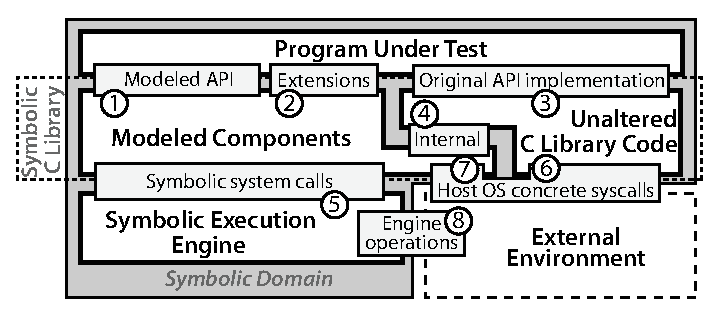
\epsfig{file=evaluation/figures/posix-model.eps, width=6in}
  \caption{Architecture of the \cnine POSIX model.}
  \label{fig:cloud9:posixmodel}
\end{figure}

\cnine builds upon the \klee symbolic execution engine, and so it inherits from \klee the mechanism for replacing parts of the C Library with model code; it also inherits the external calls mechanism.  \cnine adds the symbolic system call interface and replaces parts of the C Library with the POSIX model.  The resulting architecture is shown in Figure~\ref{fig:cloud9:posixmodel}.

Before symbolic execution starts, the \cnine system links the program under test with a special symbolic C Library.
%
We built this library by replacing parts of the existing uClibc library in \klee with the POSIX model code.  Developers do not need to modify the code of to-be-tested programs in any way to make it run on \cnine.  

In the C Library, we replaced operations related to threads, processes, file descriptors, and network operations with their corresponding model \cI, and augmented the API with \cnine-specific extensions \cII.
%
A large portion of the C Library is reused, since it works out of the box \cIII (e.g. memory and string operations).  Finally, parts of the original C Library itself use  the modeled code \cIV (e.g., Standard I/O \codebit{stdio} relies on the modeled POSIX file descriptors).

The modeled POSIX components interface with the SEE through symbolic system calls \cV, listed in Table~\ref{table:cloud9:primitives} from Section~\ref{sec:cloud9:primitives}.
%
Occasionally, the unmodified part of the C Library invokes external system calls \cVI, and the model code itself needs support from the host OS \cVII---in order to make sure the external calls do not interfere with the symbolic engine's own operations~\cVIII, such access is limited to read-only and/or stateless operations.  This avoids problems like, for instance, allowing an external \codebit{close()} system call to close a network connection or log file that is actually used by the SEE itself.

\klee uses copy-on-write (CoW) to enable memory sharing between symbolic states.
%
We extend this functionality to provide support for multiple address spaces.
%
We organize the address spaces in an execution state as \emph{CoW domains} that permit memory sharing between processes.
%
A memory object marked as shared by calling \codebit{\cninesuffix\_\allowbreak{}make\_\allowbreak{}shared} is automatically mapped in the address spaces of the other processes within the CoW domain.  Whenever a shared object is modified in one address space, the new version is automatically propagated to the other members of the CoW domain.

%%% Local Variables: 
%%% mode: latex
%%% eval: (visual-line-mode)
%%% fill-column: 1000000
%%% TeX-master: "main"
%%% End:
